\chapter{时间与距离}

\section{运动}

在这一章里我们将研究\uwave{时间}和\uwave{距离}这两个概念的某些方面。上面我们曾经强调过,物理学像所有其他科学一样是依赖于观察的,人们或许还可以说,物理科学发展到它今天这种形式在很大程度上是由于强调了要进行\uwave{定量的观察}。唯有通过定量的观察,人们才能得到定量的关系,这些关系是物理学的核心。

很多人都喜欢把伽利略在350年前所做的工作看作是物理学的开端,并且称他为第一个物理学家。在此之前,对运动的研究是一种哲学上的事情,它所根据的是人头脑中所能想象出来的一些论据。大部分的论据是由亚里士多德和其他希腊哲学家提出的,并且被认为是“已经证明”了的。伽利略采取一种怀疑的态度,关于运动他做了一个实验,这个实验主要是这样的:他让一个球沿一斜面滚下,并且观察它的运动。然而他并不只是观察而已,而且还测量了在\uwave{多长一段时间}内小球跑了\uwave{多远一段距离}。

在伽利略之前很久,人们已经很好地掌握了测量距离的方法,但是,对于时间的测量,特别是短时间的测量,还没有精确的方法。虽然伽利略后来设计了比较准确的钟(不过不像我们今天所见到的那样),但他在第一次做运动实验时是用他的脉搏来数出等间隔的时间。让我们也来做一下这个实验。

\begin{wrapfigure}{r}{0.4\textwidth}
    \centering
    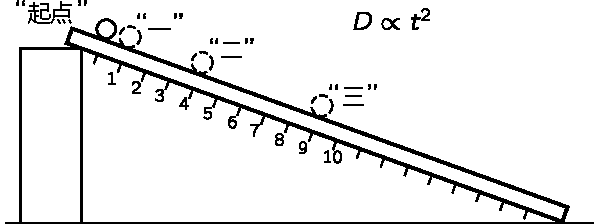
\includegraphics[width=0.35\textwidth]{Chapter5/一个小球沿着斜面滚下}
    \caption{一个小球沿着斜面滚下}
    \label{figure:一个小球沿着斜面滚下}
\end{wrapfigure}

当小球沿着轨道滚下时(图5.1),我们可以数自己的脉搏:“一…二…三…四…五…六…七…八…。”我们请一个朋友于每数一次就在小球所到达的位置上做一个小记号;然后就可以测量小球从被释放的位置开始在1个、2个或3个等等相等时间间隔内所经过的\uwave{距离}。伽利略用下面这种方法来表述\uwave{他的}观察结果:如果从小球释放的时刻算起,它的位置是在1,2,3,4,……单位时间记下的,那么这些记号离开起点的距离就正比于数1,4,9,16,……。今天我们就会这样说:距离与时间的平方成正比:
\begin{equation*}
D\propto t^2.
\end{equation*}

\uwave{运动}的研究对所有物理部门是一件基本的事,它所讨论的问题是何处与何时?


\section{时间}

让我们先来考察一下何谓\uwave{时间}。时间究竟是什么?假如我们能够找到时间的一个确切的定义那该是多好。在韦伯斯特辞典里把“一段时间(a time)”定义为“一个时期(a period)”,又把后者定义为“一段时间”。这种定义看来并不十分有用。或许我们应该说:“时间就是不发生其他事情时所发生的事。”然而这也未必使我们的理解深入。事实上(就字典的含义来说) 时间很可能是我们不能定义的事物之一。面对这个事实也许并没有什么不好。我们干脆说时间就是我们所知道的那回事:它就是我们等了多久!

不管怎样,重要的不在于我们是如何来\uwave{定义}时间,而在于我们如何来测量它 测量时间的一种方法是利用某种能以有规则的方式一再发生的事情,即某种能\uwave{周期性}发生的事情。例如,一个昼夜。昼夜似乎是一再重复出现的。然而你思索一下,也许就会问:“昼夜是否系真正周期性重复的?它们是否有规则地变化着?每一天是否都同样长?”人们肯定会有这种印象,夏天的日子比冬天的日子长。当然,在人们感到非常无聊的时候,总觉得冬天的有些日子长得可怕。你们一定会听到过有人这么说:“哎呀,这是多么长的一天!”

但是\uwave{就平均而言},日子确实大致一样长。我们有没有什么方法来检验日子——不论从一天到下一天,或者至少就其平均而论——长短相同与否?一个办法是把它同某种别的周期性现象作比较,我们来看怎样能用一个沙漏来做这种比较。如果我们让某个人昼夜站在它的旁边,每当最后一粒沙掉下之后,他就把沙漏倒转来,这样,我们用沙漏就能“创造”一个周期性的事件。

于是,我们就能计算从每天早上到下一天早上倒转沙漏的次数,这一次我们大概会发现每一“天”的“小时”数(即倒转沙漏的次数)并不相同。这样,我们就会猜疑太阳或者沙漏,或者怀疑这二者。在加以思索之后,我们或许会想到要计算从这个中午到下一个中午的“小时”数。(在这里中午的定义并不是12:00,而是指太阳在其最高点的时刻。)这一次我们将会发现,每一天的小时数都是相同的。

现在我们比较有把握认为“小时”和“昼夜”具有一种有规则的周期性,也就是说它们划分出相继的等时间间隔,虽然我们没有\uwave{证明}它们中不论那一个“确实”是周期性的。或许有人会问:是否会有某个万能者在夜间使沙漏中的流动变慢,而在白天又把它加快?我们的实验当然无法对这类问题做出回答,我们所能说的,只是发现一种事物的规则性与另一种事物的规则性相吻合而已。我们只能说把时间的\uwave{定义}建立在某种明显是周期性的事件的重复性上。


\section{短的时间}

现在我们要指出,在检验昼夜的重复性这个过程中我们获得了一个重要的副产品。这就是找到了一种比较精确地测量一天的\uwave{几分之一}的方法。亦即我们找到了一种用较小的间隔来计点时间的方法。能不能把这种过程再往前发展,从而学会测量甚至更小的时间间隔呢?

伽利略断定,只要一个摆的摆幅始终很小,那么它将总以相等的时间间隔来回摆动。如果做这样一个实验,对摆在一“小时”内的摆动次数进行比较,那么这个实验就会表明,情况确实如此。我们用这个方法可划分出一个小时的\uwave{几分之一}。假如我们利用一个机械装置计点摆动次数,并且保持摆动进行下去,那么就得到了我们祖父一代所用的那种摆钟。

让我们约定,如果我们的摆一小时内振动3600次(并且如果一天有24个这样的小时),那么我们就称每一摆动的时间为1“秒”。这样,就把原来的时间单位分成大约$ 10^5 $个部分。我们可以应用同样的原理把秒分成更加小的间隔。你们可以理解,制造一个能够走得任意快的机械摆是不现实的,但是我们现在能够制造一种称为振荡器的\uwave{电学摆}。这种电学摆能提供周期很短的摆动。在这种电子振荡器中,是电在来回振动,其方式与摆锤的摆动方式相类似。

我们可以制造一系列这种电子振荡器,每一个的周期要比前一个减小10倍。每一个振荡器可用前一个较慢的振荡器这样来“定标”,即数出较慢的振荡器振动一次时它所振动的次数。当我们的钟的振动周期小于一秒的几分之一时,如果没有某种辅助装置以扩展我们的观察能力,那就无从计点振动的次数。这种装置之一是电子示波器,它的作用就像一种供短的时间用的“显微镜”。这个装置在荧光屏上画出一幅电流(或电压)对时间的图像。将示波器依次与我们的系列中相继的两个振荡器相连,它就先显示出一个振荡器中的电流图像,然后显示出另一个振荡器中的电流图像,从而得到如图5.2所示的两幅图像。这样,我们就很容易测出较快的振荡器在较慢的振荡器的一个周期中振动的次数。

\begin{figure}
    \centering
    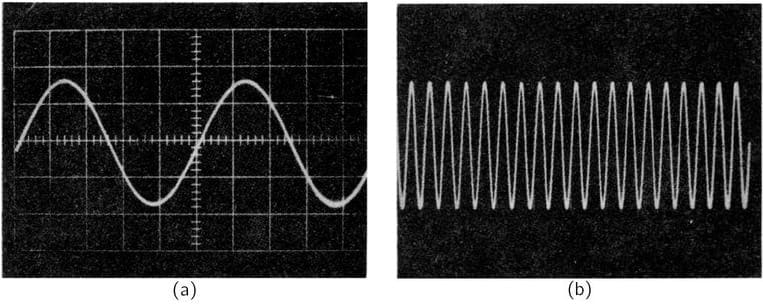
\includegraphics[width=0.8\textwidth]{Chapter5/示波器屏上的两个图象}
    \caption{\footnotesize 示波器屏上的两个图象。在(a)中,示波器与一个振荡器相连接;在(b)中,它与另一个其周期只有前者十分之一的振荡器相连接。}
    \label{figure:示波器屏上的两个图象}
\end{figure}

利用现代电子技术,已经制造出周期短到大约$ 10^{-12} $秒的振荡器,并且可以按照前面描述的那种比较方法用我们的标准时间单位——秒来予以定标。近年来,随着“激光器”或光放大器的发明和完善,已能制造周期甚至比$ 10^{-12} $秒更短的振荡器了,但是还不能用上述那些方法来予以定标,虽然毫无疑问,这在不久期间一定能够做到。

比$ 10^{-12} $秒还短的时间已经测量出来,但用的是另一种测量技术。事实上,这里所用的是“时间”的另一种\uwave{定义}。一个方法是观察发生在运动物体上的两个事件之间的\uwave{距离}。例如,假定有一辆行驶的汽车把它的车灯先开亮,然后再关掉。如果我们知道车灯开、关的\uwave{地点},以及车速,那么我们就能求出灯开的时间有多长。这段时间就是灯开时所通过的距离除以汽车的车速。

近几年来,正是这种技术被用来测量$\pi^0$介子的寿命。$\pi^0$介子在感光乳剂中产生并在其中留下微细的踪迹,用显微镜观察这些踪迹时,人们就可看到,平均而言一个$\pi^0$介子(认为它以近于光速的某个速度运动)在蜕变之前大约走过了$ 10^{-7} $米的距离,所以它的寿命总共只有大约$ 10^{-16} $秒。但是必须着重指出,这里我们用了一个与前稍有不同的“时间”的定义。然而,只要在我们的理解方面不出现任何不协调的地方,那么我们就觉得有充分的信心认为这些定义是足够等效的。

在把我们的技术——而且如有必要也把我们的定义——进一步加以扩展之后,就能推断更快物理事件的持续时间,我们可以谈论原子核振动的周期,以及第二章中提到过的那种新发现的奇异共振态(粒子)的寿命。它们的全部寿命只不过占$ 10^{-24} $秒的时间,大致相当于光(它以我们已知的最快速度运动)通过氢原子核(这个已知的最小物体)所花的时间。

那么,再短的时间呢?是不是还存在尺度更小的“时间”?如果我们不能够测量——或者甚至合理地去设想——某些发生在更短时间内的事情,那么要谈论更短的时间是否还有任何意义?可能没有意义。这是一些尚未解决的、但你们会提出的、而且也许在今后二十或三十年内才能回答的问题。


\section{长的时间}

我们现在来考虑比一昼夜还长的时间。要测量较长的时间很容易,我们只要数一数有几天就是——只要旁边有人在做这种计数的工作。首先我们发现,自然界里存在着另一个周期性,即年,一年大约等于365天。我们还发现,自然界有时也为我们提供了计算年的一些东西,例如树木的年轮或河流底部的沉积物。在某些情况下,我们就能利用这些自然界的时间标记来确定从发生某种事件以来所经历的时间。

当我们不能用计算年的方法来测量更长的时间时,那就必须寻找其他的测量方法。最成功的方法之一是把放射性材料作为一只“钟”来使用。在这种情况下,并不出现像昼夜或摆那样周期性的事件,但是有一种新的“规则性”。我们发现,某种材料的样品,当它的年龄每增加一相同的数值时,它的放射性就减少一相同的\uwave{分数}。假如我们画一张图来表示所观察到的放射性作为时间(比方以天来计算)的函数,那么我们就得到如图5.3所示的一条曲线。我们看到,如果放射性在$ T $天内减少到一半(称为“半衰期”),那么它在另一个$ T $天内就减少到四分之一等等。在任一时间间隔$ t $内共包含了$ t/T $个半衰期,而在这段时间$ t $后尚剩下的部分则是$ (\tfrac{1}{2})^{t/T} $。

\begin{table}[!ht]
    \centering
    \caption{时间}
    \setlength{\tabcolsep}{7mm}{
    \begin{tabular}{|cc|cc|}
    \hline
        年 & 秒 & ~ & 等效平均寿命物质 \\ \hline
        ~ & ~ & ?????? & ~ \\ \hline
        ~ & $10^{18}$ & 宇宙的年龄 & $U^{238}$ \\ \hline
        $10^9$ & ~ & 地球的年龄 & ~ \\ \hline
        ~ & $10^{15}$ & ~ & ~ \\ \hline
        $10^6$ & ~ & 最早的人 & ~ \\ \hline
        ~ & $10^{12}$ & 金字塔的年龄 & ~ \\ \hline
        ~ & ~ & ~ & $Ra^{226}$ \\ \hline
        $10^3$ & ~ & 美国的历史 & ~ \\ \hline
        ~ & $10^9$ & 一个人的寿命 & $H^3$ \\ \hline
        ~ & $10^6$ & 一天 & ~ \\ \hline
        ~ & $10^3$ & 光从太阳射到地球 & 中子 \\ \hline
        ~ & 1 & 一次心跳 & ~ \\ \hline
        ~ & $10^{-3}$ & 声波的周期 & ~ \\ \hline
        ~ & $10^{-6}$ & 无线电波的周期 & $\mu$介子 \\ \hline
        ~ & ~ & ~ & $\pi^{\pm}$介子 \\ \hline
        ~ & $10^{-9}$ & 光通过1ft的距离 & ~ \\ \hline
        ~ & $10^{-12}$ & 分子转动的周期 & ~ \\ \hline
        ~ & $10^{-15}$ & 原子振动的周期 & ~ \\ \hline
        ~ & ~ & ~ & $\pi^0$介子 \\ \hline
        ~ & $10^{-18}$ & 光经过一个原子 & ~ \\ \hline
        ~ & $10^{-21}$ & 核振动的周期 & ~ \\ \hline
        ~ & $10^{-24}$ & 光经过一个原子核 & 奇异粒子 \\ \hline
        ~ & ~ & ????? & ~ \\ \hline
    \end{tabular}}
\end{table}

如果我们知道一块材料比如说一块木料,在它形成时其中含有数量为$ A $的放射性物质,而用直接测量我们发现它此刻的量为$ B $,那么只要解方程
\begin{equation*}
(\frac{1}{2})^{t/T}=\frac{B}{A}
\end{equation*}
就能计算这一物体的年龄$ t $。

\begin{wrapfigure}{r}{0.45\textwidth}
    \centering
    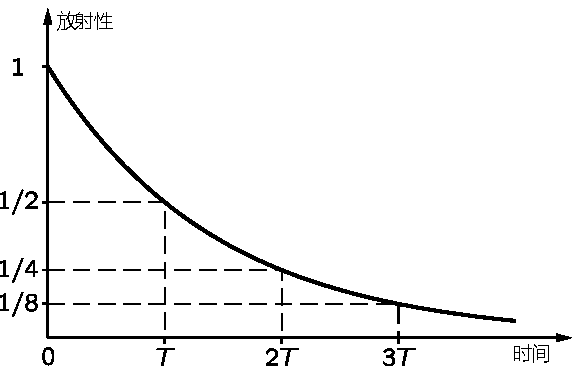
\includegraphics[width=0.35\textwidth]{Chapter5/放射性随时间而减少}
    \caption{\footnotesize 放射性随时间而减少。在每一个“半衰期”$ T $中,放射性都减少一半}
    \label{figure:放射性随时间而减少}
\end{wrapfigure}
幸运的是,在某些情况中,我们可以知道物体在形成时它所包含的放射性总量。比如说我们知道空气中的二氧化碳含有某一确定小量的放射性碳同位素C$ ^{14} $(它由于宇宙线作用而连续不断地得到补充),如果我们测量一个物体的碳的总含量,并且知道这个总含量的某一分数原来是放射性的C$ ^{14} $,那么,我们就知道上述公式中所要用到的那个开始时的总含量$ A $ 。碳14的半衰期是5000年,通过仔细的测量我们测出经20个左右的半衰期后所余留下来的数量。因此,我们就能够确定生长于100,000年以前那样古老的有机体的年代。

我们很想知道,并且认为也能知道比之更老的那些事物的寿命。许多有关这方面的知识,我们是通过测量具有不同半衰期的其他放射性同位素而得到的。如果我们用一种半衰期更长的同位素来进行测量,那么就能测得更长的时间。例如,铀有一种同位索,它的半衰期大约为$ 10^9 $年,所以如果有一种物质在它$ 10^9 $年前形成时就含有这种铀,那么今天这种铀就只剩下一半。当铀蜕变时,它变成了铅。设想有一块岩石,它是在很久以前通过某种化学过程形成的。铅由于具有与铀不同的化学性质,它将出现在岩石的一个部分中,而铀则出现在岩石的另一部分中。铀和铅将互相分开。如果我们今天来考察那块岩石将发现在那种应该只有铀存在的地方,现在有某一分数的铀和某一分数的铅,通过对这两个分数的比较;我们就能说出百分之几的铀已消失并且变成了铅。利用这个方法,有些岩石的年龄被测定为几十亿年。这个方法的一个推广便是不用特定的岩石,而是着眼于海洋中的铀和铅,并且对整个地球取其平均值。用这个推广了的方法(在过去几年中)曾测得地球本身的年龄为大约55亿年。

人们发现,地球的年龄与掉到地球上的陨石(也是用铀方法测定的)的年龄是相同的,这是一件令人鼓舞的事情。看来,地球是由漂游在太空中的岩石形成的,而陨石很可能就是遗留下来的那些物质的残片。在50亿年前的某个时候,宇宙开始形成。现在人们认为,至少我们这部分宇宙起源于大约100或120亿年之前。我们不知道在此之前发生过什么事情。事实上我们又可以提出来问:这个问题是否有任何意义?更早的时间是否有任何意义?


\section{时间的单位和标准}

我们在前面实际上已表明了,如果从时间的某个标准单位,比如一天或一秒出发,并把所有其他的时间表示为这个单位的倍数或分数,那么将十分方便。然而,我们将用那个单位作为我们的时间基本标准呢?是否用人的脉搏跳动?如果我们比较各人的脉搏,那就会发现它们之间似乎差别很大。如果比较两只钟,则发现它们的变化不那么大。于是你们会说:好,就让我们采用钟吧!但是用谁的钟呢?有个故事讲到一个瑞士男孩,他想使他所在的镇上所有的钟在正午时刻都同时敲响,所以他就跑来跑去,穿家过院,想使人人相信这样做的好处。每个人都想,如果他的钟在正午敲响时,其他钟也全都敲响的话,这该是一个多好的主意呀!然而要决定谁的钟应该取作标准,这倒是一件难事。幸运的是,我们大家都同意用一只钟,即地球。在很长一段时间里,人们把地球的自转周期当作时间的基本标准。但是当测量越来越变得精确的时候,人们发现,用最好的钟来进行测量,地球的转动也不是严格周期性的。我们有理由相信,这些“最好”的钟是精确的,因为它们彼此之间是相符的。由于种种理由,我们现在认为,有些天要比另一些天长,有些天要比另一些天短,平均而论,地球的自转周期是随着一个世纪一个世纪的过去而变长了一点的。

直到晚近以前,我们还没有找到任何一个比地球的周期好得多的标准,所以把所有的钟同一天的长度联系了起来,而把一秒规定为一个平均日的$  1/86400$。最近我们对自然界中某些振荡器获得了一些经验。我们现在相信,这些振荡器可以当作比地球更稳定的时间参考物。而且,它们也是基于一个大家都能采用的自然现象。这就是所谓的“原子钟”。它的基本的内在周期,就是原子振动的周期,这种振动对于温度或任何其他外界影响都不十分敏感。原子钟能使时间的精确度达到$ 10^9 $分之一,或者比之更高。在过去二年中,哈佛大学的拉姆齐(N.Ramsay)教授研制了一种改进的原子钟,它是依靠氢原子的振动而工作的。拉姆齐认为,这种钟比其他原子钟精确100倍。现在他正在对之作测量,这些测量将表明他的说法是否正确。

既然现在有可能制作远比天文时间精确的钟,那么我们可以预期,科学家们不久就会一致同意采用许多原子标准钟中的一种来定义时间单位\footnote{1967年的第十三届国际计量大会已通过决议将时间单位“秒”的定义改为:“一秒等于铯133原子基态的两个超精细能级之间跃迁的辐射周期的9,192,631,770倍。”——译者注。}



\section{长的距离}
现在我们转到\uwave{距离}的问题上来。事物有多远,或者有多大?人们都知道测量距离的方法是选用一种长度单位再加上计数,例如可以用尺或拇指边量边数。那么怎样来量比较小的东西呢?怎样把距离分小呢?这与我们将时间分小一样,我们同样取一个较小的单位,然后数出这个单位组合成一个较长单位时所需的数目。这样我们就能测量越来越小的长度。

\begin{wrapfigure}{r}{0.45\textwidth}
    \centering
    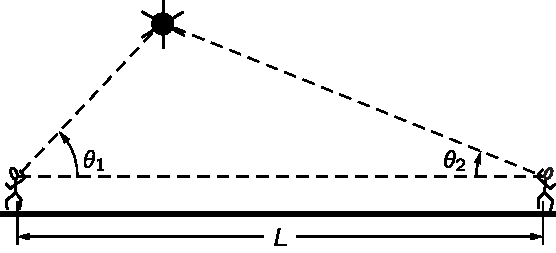
\includegraphics[width=0.35\textwidth]{Chapter5/用三角法测定人造卫星的高度}
    \caption{用三角法测定人造卫星的高度}
    \label{figure:用三角法测定人造卫星的高度}
\end{wrapfigure}
但是我们并不总是把距离理解为用米尺量。得的结果。仅仅用一根米尺是难以测量两个山顶之间的水平距离的。我们曾经凭经验发现可以用另一种方式来测量距离:即用三角法。虽然这意味着我们实际上对距离用了一个不同的定义,但当它们可以一起应用时,就应是彼此相一致。空间或多或少有点像欧几里得所设想的那个样子,所以距离的这两种定义是一致的。既然它们在地球上相一致,那就使我们充满信心可用三角法来测量更大的距离。例如,我们当时曾用三角法测定了第一颗人造卫星的高度(图5.4)。我们测得的高度约有$ 5\times 10^5$米。如果测量得更仔细一点,则用同样的方法可以测出地球到月球的距离;安放在地球上两个不同地点的两个望远镜,将会告诉我们所需要的两个角度。用这种方法我们求得月球离我们有$ 4 \times 10^8 $米远。

对于太阳,我们不能这样做,或者至少到现在没有人能够这样做。由于我们不能相当精确地对准太阳上一个特定的点,从而不能精确地测出两个角度,所以无法测出到太阳的距离。然而如何来测量这个距离呢?我们必须将三角法这个观念加以引伸。我们可以通过天文观察方法来测量所有行星出现的位置之间的相对距离,从而得到一幅有关太阳系的图像,能显示每个行星间的相对距离,但都不是绝对距离。因此需要测出一个\uwave{绝对}距离,而这种绝对测量已用几种方法得到,其中直到最近以前还认为最精确的一个是测出地球到爱神星的距离。爱神星是一个时常靠近地球的小行星。如果对这个小天体应用三角法,就能得到一个所需要的比例尺度。由于知道了其他天体的相对距离,我们就能说出它们之间的绝对距离,例如地球到太阳,或地球到冥王星的绝对距离。

\begin{figure}[htbp]
    \centering
    \begin{minipage}[t]{0.4\textwidth}
        \centering
        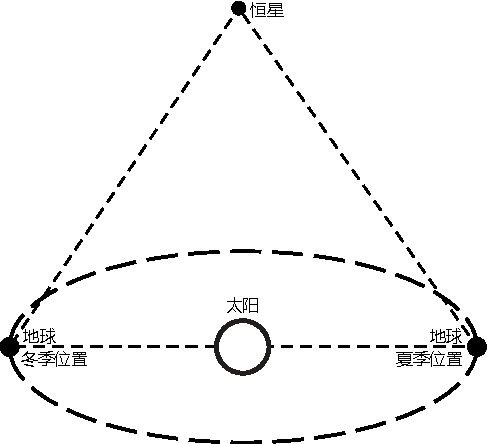
\includegraphics[width=5cm]{Chapter5/三角法测量恒星距离}
        \caption{\footnotesize 利用地球轨道的直径作为基线,可以用三角法测量靠近地球的恒星的距离}
    \end{minipage}
    \begin{minipage}[t]{0.4\textwidth}
        \centering
        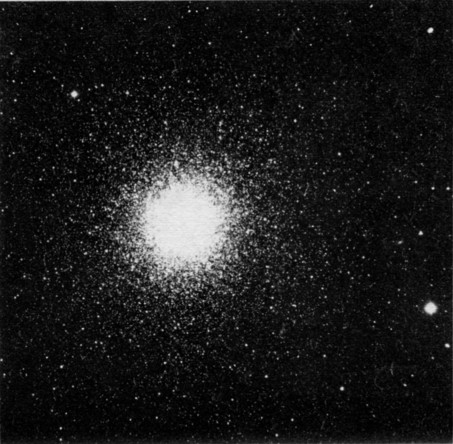
\includegraphics[width=5cm]{Chapter5/靠近我们银河系中心的一个星团}    
        \caption{\footnotesize 靠近我们银河系中心的一个星团,其中各恒星与地球的距离为30,000光年,或约$ 3\times 10^{20} $米}
    \end{minipage}
\end{figure}

去年,我们在有关太阳系的比例尺度的了解上获得了巨大的进展。喷气推进实验室用直接的雷达观察非常精确地测定了地球到金星的距离。当然,这只是另外一种由推测而得到的距离。我们说,我们知道光传播的速度(因而这也是雷达波传播的速度),并且假定,在地球与金星之间无论何处这个速度都相同。那么,在发射无线电波并测得电波返回的时间,我们就能从\uwave{时间}来推测\uwave{距离}。这确实是距离测量的另一种定义。

可是我们如何来测量一个更遥远的恒星的距离呢?幸运的是,我们可以回到三角法上来,因为地球绕太阳公转,而这种转动就为测量太阳系外的恒星距离提供了一条基线。假如我们在夏天和冬天用望远镜对准一颗恒星,那么我们可以期望能足够精确地测出这两个角度,从而能测出地球到恒星的距离。

如果恒星离得太远而不能应用三角法时又怎么办?天文学家总是在发明测量距离的新方法。例如,他们发现,从恒星的颜色可以估计它的大小和亮度。他们测定了许多靠近地球的恒星——这些恒星的距离已用三角法测得——的颜色和内在亮度,并且发现在恒星颜色和内在亮度(在大多数情况中)之间存在着一个平滑的关系,如图5.5所示。如果现在测出了一个遥远恒星的颜色,那就可以用颜色—亮度关系来确定这个星体的内在亮度,在测量了我们地球上看来这颗恒星有多亮(或许应该说有多\uwave{暗})之后,我们就可以计算它有多远(对于一个给定的内在亮度,其表观亮度是随距离的平方而减小的)。对称为球状星团的一群恒星作测量后,所得的结果很好地证实了这种星际距离测量方法的正确性。图5.6是这样一群恒星的一张照片。只要看一下照片,人们就会相信这些恒星都聚集在一起。用颜色—亮度关系这个测量距离的方法得到了同样的结果,

\begin{figure}[htbp]
    \centering
    \begin{minipage}[t]{0.4\textwidth}
        \centering
        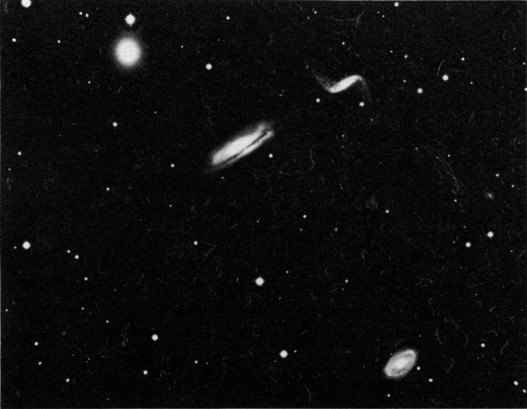
\includegraphics[width=6cm]{Chapter5/和我们银河系一样的一个螺旋银河系}
        \caption{\footnotesize 和我们银河系一样的一个螺旋银河系,假定它的直径与我们银河系相近,那么我们从它的表观大小就能算出它的距离。它离地球约3000万光年(即$ 3\times 10^{23} $米)}
    \end{minipage}
    \begin{minipage}[t]{0.4\textwidth}
        \centering
        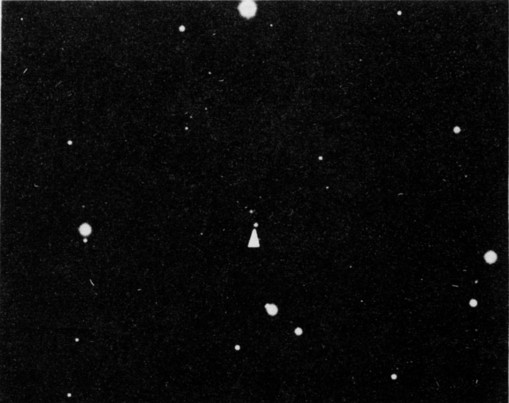
\includegraphics[width=6cm]{Chapter5/牧夫座中的3c295}    
        \caption{\footnotesize 最现代化的200英寸望远镜拍摄的最远天体——牧夫座中的3C295(用箭头标出)}
    \end{minipage}
\end{figure}
对许多球状星团进行研究之后使我们得到另一些重要信息。人们发现,在天空的某一部分有许多这样的星团高度集中在一起,而且其中大部分离地球的距离大致相同。把这个信息和其他证据结合起来,就能断定,星团的这个集中处就是我们所在银河系的中心。于是我们就知道到银河系中心的距离——大约为$ 10^{20} $米。

知道了我们自己所在银河系的大小,我们就有了一把测量更大距离——也就是到其他银河系的距离——的钥匙。图5.7是一副形状与我们的银河系颇为相同的一个银河系的照片。它的大小可能也和我们的相近。(另外的一个证据支持了这种想法,即所有银河系都有相近的大小。)假如确实如此,那我们就能说出它的距离,我们测量它在天空中的张角,又知道了它的直径,于是就能算出它的距离——这又是三角法!

新近用巨大的帕洛马望远镜获得了极其遥远的一些银河系的照片,图5.8是其中的一张。现在人们认为,这样的一些银河系大约处在从地球到我们宇宙界限——$ 10^{26} $米处——一半的地方。$ 10^{26} $米是我们能想象的最大最大距离!


\section{短的距离}
现在我们考虑一下小的距离。把一米分小是很容易的,把一米划分成一千个相等的间隔并没有多大困难。用相似的方法(利用一架好的显微镜),我们能够把1毫米分成一千等分,构成微米(一米的百万分之一)这样的尺度,但这要稍微困难一些。要继续分成更小的尺度则很困难,因为我们“看不见”一个比可见光波长(大约$ 5\times 10^{-7} $还要小的物体。

\begin{wrapfigure}{l}{0.4\textwidth}
    \centering
    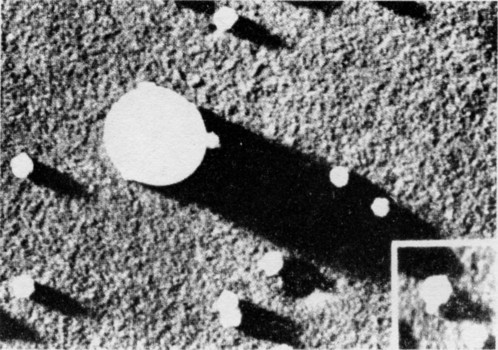
\includegraphics[width=0.35\textwidth]{Chapter5/某些病毒分子的电子显微镜图}
    \caption{\footnotesize 某些病毒分子的电子显微镜图。“大的”球是为定标用的,且已知其直径为$ 2\times 10^{-7} $米(2000 Å)}
    \label{figure:某些病毒分子的电子显微镜图}
\end{wrapfigure}
然而我们毋须停止在我们看得见的东西上,依靠电子显微镜,我们能用拍照方法来对更小的尺度(比方说一直到$ 10^{-8} $米)继续这个划分过程(图5.9)。

用间接的测量,即用一种显微镜规模的三角法,我们能对越来越小的尺度继续进行测量。首先我们从观察波长短的光(X射线)如何在间隔为已知的标记所组成的图样上被反射的情况,确定光振动的波长。然后从同样的光在一块晶体上所散射的图样,我们就能确定原子在晶体中的相对位置,所得结果与化学方法确定的原子间距离相符合。用这种方法我们发现原子的直径约为$10^{-10}$米。

典型的原子大小约为$10^{-10}$米,而原子核的大小为$10^{-15}$米,其间相差$10^5$倍!可见原子与原子核之间在物理大小上存在一个很大的“空隙”。对原子核的大小来说,用另一种测量方法比较方便。我们测量的是它的\uwave{表观面积}$\sigma$,称之为有效截面。如果要知道半径,则可从$\sigma=\pi r^2$求得,因为原子核是近似球形的。

核的截面可以这样来测量,使一束高能粒子通过某种材料的一块薄板,然后观察没有通过薄板的粒子数,这些高能粒子通常会穿过薄薄的电子云,而只有当它们碰上了质量集中的原子核时,才会被阻止或者被偏转。假设我们有一块1厘米厚的材料,其中大约有$10^8$个原子核。但原子核如此之小,以致一个核恰好位于另一个核的背后的机会是很小的。我们可以\uwave{设想},这种情况的一个高度放大的图像——沿着粒子束看去时——犹如图5.10所示。

\begin{wrapfigure}{r}{0.4\textwidth}
    \centering
    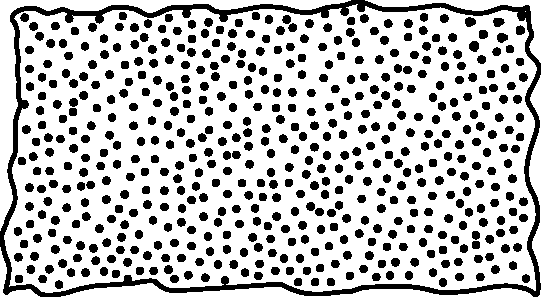
\includegraphics[width=0.35\textwidth]{Chapter5/一块厚1厘米的碳设想的图像}
    \caption{\footnotesize 在只观察核的时候,通过一块厚1厘米的碳所见到的那个设想的图像}
    \label{figure:一块厚1厘米的碳设想的图像}
\end{wrapfigure}
一个很小的粒子在通过物质时能打在一个核上的概率,正好等于其中所有核的剖面所占的总面积除以这幅图上的总面积。假定我们知道在这块板的面积$A$中有$N$个原子(当然,每个原子只有一个核),那么被这些核所“覆盖”的面积和总面积之比就等于$N \sigma / A$。现在设粒子束中射到薄板的粒子数为$n_1$,从薄板另一边射出的粒子数为$n_2$。这样,\uwave{没有} 通过薄板的粒子数和射出的粒子数之比为$(n_1-n_2)/n_1$,它们应该正好等于被覆盖面积和总面积之比。于是从等式\footnote{只有当核所覆盖的面积是总面积的一个很小分数,即$(n_1-n_2)/n_1$远比1小时,这一等式才正确。否则我们必须对有些核将部分地为其前面的核所挡住这样的情况进行校正。}
\begin{equation*}
\pi r^2=\sigma=\frac{A}{N}\,
(\frac{n_1-n_2}{n_1})
\end{equation*}
就能获得核的半径。

从这样一种实验我们得出核的半径大约为$10^{-15}$米的一到六倍。$10^{-15}$米这个长度单位称为\uwave{费米},以纪念著名的物理学家费米(1901~1958)。

\begin{table}[!ht]
    \centering
    \setlength{\tabcolsep}{13mm}{
    \begin{tabular}{|cc|c|}
    \hline
        光年 & 米 & ~ \\ \hline
        ~ & $10^{27}$ & ?????? \\ \hline
        $10^9$ & ~ & 宇宙的边缘 \\ \hline
        ~ & $10^{24}$ & ~ \\ \hline
        $10^6$ & ~ & 到最邻近的银河系 \\ \hline
        ~ & $10^{21}$ & ~ \\ \hline
        $10^3$ & ~ & 到银河系中心 \\ \hline
        ~ & $10^{18}$ & ~ \\ \hline
        1 & ~ & 到最近的恒星 \\ \hline
        ~ & $10^{15}$ & ~ \\ \hline
        ~ & ~ & 冥王星的轨道半径 \\ \hline
        ~ & $10^{12}$ & ~ \\ \hline
        ~ & ~ & 到太阳 \\ \hline
        ~ & $10^{9}$ & ~ \\ \hline
        ~ & ~ & 到月球 \\ \hline
        ~ & $10^{6}$ & ~ \\ \hline
        ~ & ~ & 人造卫星高度 \\ \hline
        ~ & $10^{3}$ & ~ \\ \hline
        ~ & ~ & 电视塔高度 \\ \hline
        ~ & $1$ & 一个孩子的高度 \\ \hline
        ~ & $10^{-3}$ & ~ \\ \hline
        ~ & ~ & 一粒盐 \\ \hline
        ~ & $10^{-6}$ & ~ \\ \hline
        ~ & ~ & 病毒 \\ \hline
        ~ & $10^{-9}$ & ~ \\ \hline
        ~ & ~ & 原子半径 \\ \hline
        ~ & $10^{-12}$ & ~ \\ \hline
        ~ & $10^{-15}$ & 原子核半径 \\ \hline
        ~ & ~ & ?????? \\ \hline
    \end{tabular}}
\end{table}

如果我们进到更小的距离,那么将会发生什么呢?能不能测量更小的距离?这样的问题现在还不可能回答。有人提出这种看法,认为迄今尚未解决的核力之谜,只有在对这样小的距离下的我们关于空间或测量的观念进行某些修正以后才能解开。

人们也许会想到,用某些自然长度来作为我们的长度单位——比如说地球的半径或者它的某一部分——倒是一个很好的意见。米之取作为单位只是出于这样的考虑,它被定义为地球半径的$(\pi/2)\times10^{-7}$倍。但是,用这种方法来规定长度单位,既不方便,也不很准确。很长时间以来国际上大家约定:一米的定义是保持在法国一个特殊实验室中的一根棒上两条刻线之间的距离。不久前人们认识到这个定义既未精确到足以使之有用,也不像人们所希望的那样稳定或普遍。近年来正在考虑采用一个新的定义,即选定一根光谱线,把大家一致同意的它的波长的(任意)倍数作为长度的单位。

距离测量和时间测量的结果有赖于观察者。两个作相互运动的观察者在测量看来似乎是同一个的事物时,将不会得到同样的距离和时间。距离和时间间隔随着测量时所用的坐标系(或“参考系”)不同而有不同的大小。我们将在后面的一章中详细地研究这个问题。

完全精密的距离测量或时间测量是为自然规律所不允许的。我们前面已经提到,在测量一个物体的位置时,误差至少要像
\begin{equation*}
\Delta x\geq\frac{\hbar}{2\Delta p},
\end{equation*}
那样之大,其中$\hbar$是一个称为“普朗克常数”的很小的量,而$\Delta p$是我们在测量物体的位置时,对它的动量(质量乘以速度)的知识上的误差。我们也曾提到,位置测量的不确定性是与粒子的波动本质有关的。

空间和时间的相对性意味着时间的测量也有一个实际由
\begin{equation*}
\Delta t\geq\frac{\hbar}{2\Delta E},
\end{equation*}
给出的最小误差,其中$\Delta E$是我们在测量一个过程的时间时,对它的能量的知识上的误差。如果我们要\uwave{更}精确地知道某个事件\uwave{何时}发生,那就只能对发生了什么知道得更少一点,因为我们对其所含能量的知识减少了。时间的不确定性也是与物质的波动本质有关的。
